\begin{figure}[htbp]
  \centering
  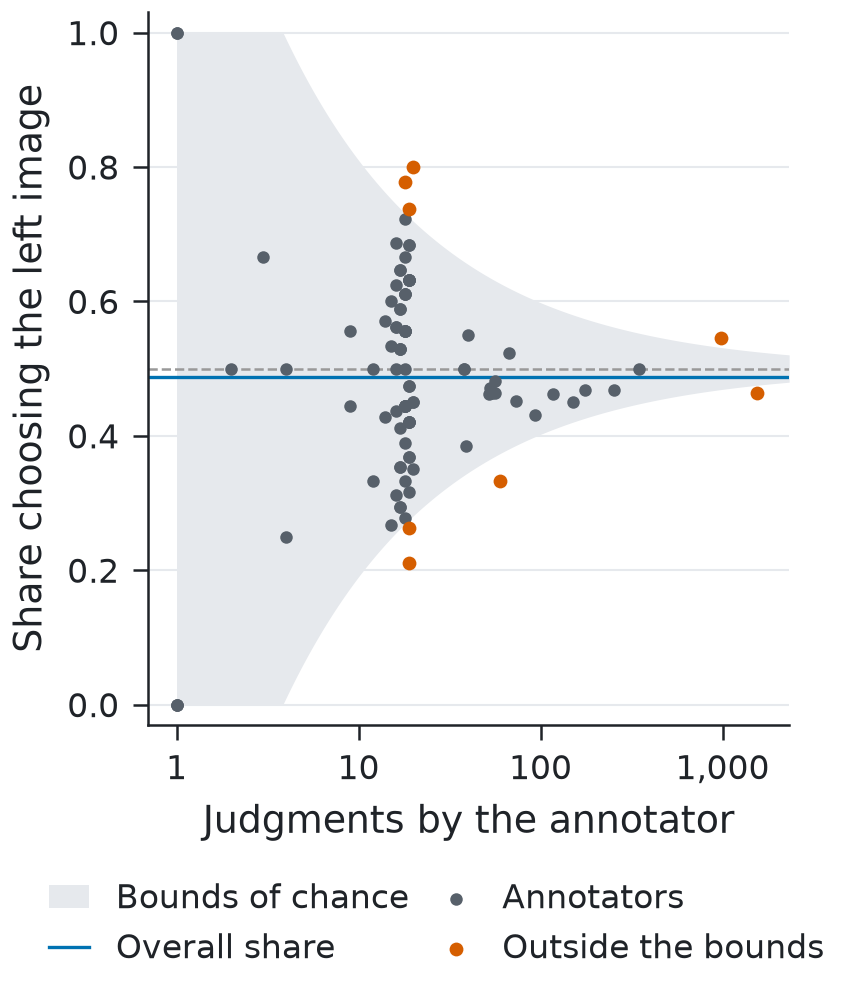
\includegraphics[width=7.20cm]{figures/position_bias_funnel.png}
  \caption{Position bias by annotator: each annotator's share of judgments that chose the image shown on the left, against their number of judgments (on a logarithmic scale). With no preference for either side, a share falls within the grey bounds by chance alone 95\% of the time: one half $\pm\ 1.96\sqrt{1/4n}$ for $n$ judgments, narrower as the judgments grow. An annotator outside them (in vermillion) leans to one side more than chance would give, which is when the 95\% (Wilson) interval of their share leaves out one half. The solid line is the overall share, the dashed one one half. The overall share, 0.488 [0.475, 0.501], is within chance. Eight of the 101 annotators lean beyond chance, where about five would by chance alone; the two most prolific lean in opposite directions: one chose the left image in 46.4\% of 1,549 judgments, the other in 54.5\% of 982.}
  \label{fig:position_bias_funnel}
\end{figure}
